% #############################################################################
% This is Chapter 3
% !TEX root = ../main.tex
% #############################################################################
% Change the Name of the Chapter i the following line
\fancychapter{Related Work}
\cleardoublepage
% The following line allows to ref this chapter
\label{chap:architecture}

This chapter reviews existing work in aerial image segmentation datasets, referring segmentation models, and related approaches.

% #############################################################################
\section{Aerial Image Segmentation Datasets}

Overview of datasets used for aerial imagery analysis and referring segmentation tasks.

[Reference to iSAID dataset] % \cite{placeholder_isaid}

\begin{figure}[htbp]
\centering
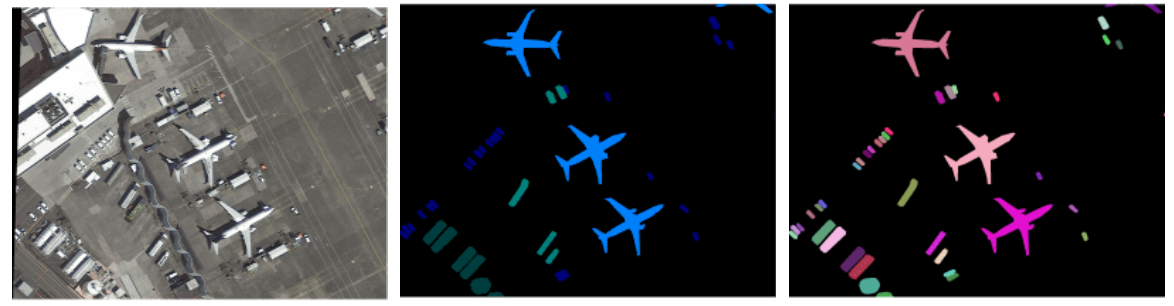
\includegraphics[width=0.8\textwidth]{Images/isaid_examples.png}
\caption{iSAID dataset examples showing instance segmentation and semantic segmentation annotations for aerial imagery.}
\label{fig:isaid_examples}
\end{figure}

[Reference to LoveDA dataset] % \cite{placeholder_loveda}

\begin{figure}[htbp]
\centering
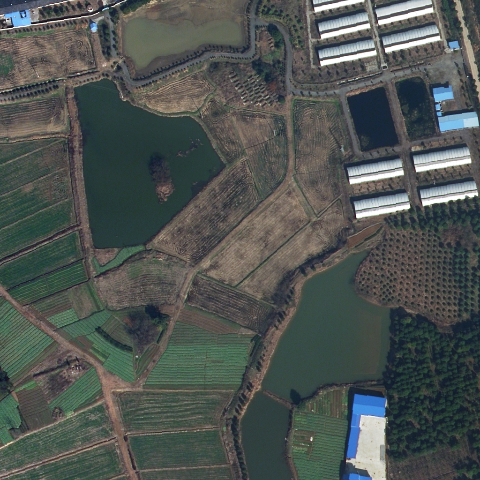
\includegraphics[width=0.8\textwidth]{Images/loveda.png}
\caption{LoveDA dataset examples showing semantic segmentation annotations for land use and land cover classification in aerial imagery.}
\label{fig:loveda_examples}
\end{figure}

[Reference to Potsdam and Vaihingen semantic segmentation datasets] % \cite{placeholder_potsdam} \cite{placeholder_vaihingen}

[Reference to RefSegRS referring segmentation dataset] % \cite{placeholder_refsegrs}

[Reference to RRSIS-D dataset] % \cite{placeholder_rrsis_d}

\begin{figure}[htbp]
\centering
\subfigure[RefSegRS dataset example samples.]{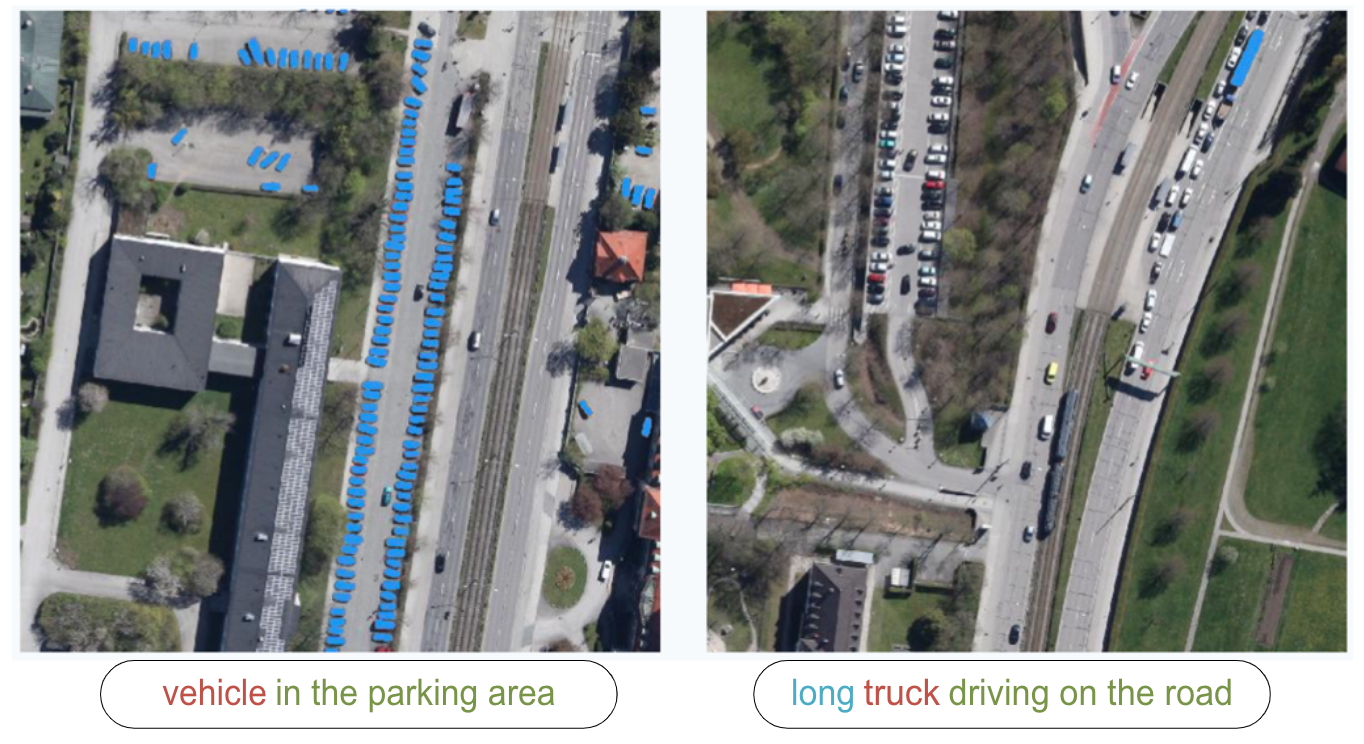
\includegraphics[width=0.45\textwidth]{Images/refsegrs.png}\label{fig:refsegrs}}
\hfill
\subfigure[RRSIS-D dataset example samples.]{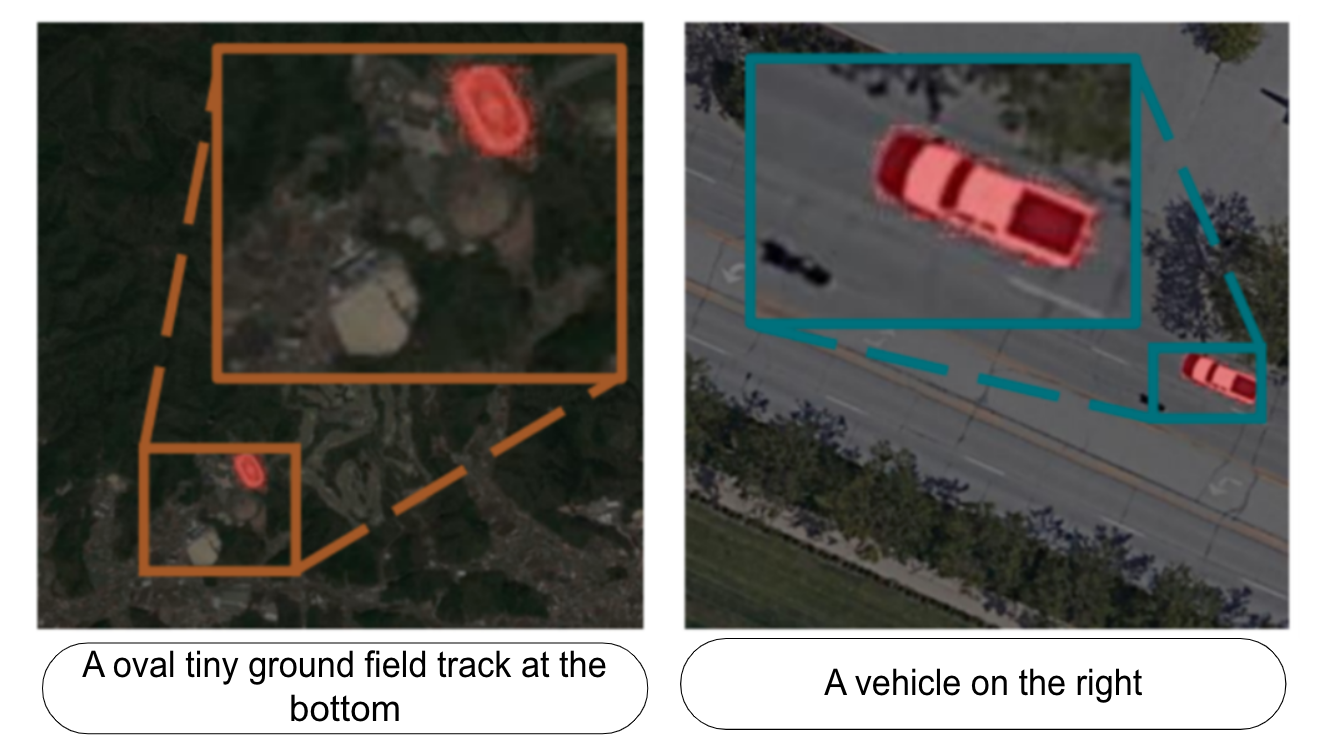
\includegraphics[width=0.45\textwidth]{Images/rrsisd.png}\label{fig:rrsisd}}
\caption{Examples from aerial referring segmentation datasets showing diverse referring expressions with corresponding images and ground truth masks.}
\label{fig:aerial_datasets}
\end{figure}

[Reference to NWPU-Refer dataset] % \cite{placeholder_nwpu}

[diagram for NWPU-Refer dataset example samples]

\begin{table}[htbp]
\centering
\caption{Remote Sensing Dataset Comparison}
\label{tab:dataset_comparison}
\begin{tabular}{@{}lllll@{}}
\toprule
\textbf{Feature} & \textbf{RefSegRS} & \textbf{iSAID} & \textbf{RRSIS-D} & \textbf{NWPU-Refer} \\
\midrule
Size & 4,420 triplets & 655,451 instances & 17,402 triplets & 15,003 images \\
Source & SkyScapes & DOTA (re-ann.) & RSVGD & Multi-source global \\
Annotation & Manual & Professional & Semi-auto (SAM) & Manual \\
Resolution & Limited & High res. & 800×800 fixed & 1024-2048px \\
Focus & RRSIS & Instance Seg. & RRSIS & RRSIS \\
Categories & - & 15 & 20 & 32 \\
Attributes & 3 & - & 7 & 6 dimensions \\
\bottomrule
\end{tabular}
\end{table}

\begin{table}[htbp]
\centering
\caption{Dataset Split Statistics}
\label{tab:dataset_splits}
\begin{tabular}{@{}llllll@{}}
\toprule
\textbf{Dataset} & \textbf{Total} & \textbf{Training} & \textbf{Validation} & \textbf{Test} & \textbf{Unit} \\
\midrule
RefSegRS & 4,420 & 2,172 (49.1\%) & 431 (9.8\%) & 1,817 (41.1\%) & expressions \\
iSAID & 2,806 & 1,403 (50.0\%) & 468 (16.7\%) & 935 (33.3\%) & images \\
RRSIS-D & 17,402 & 8,701 (50.0\%) & 3,480 (20.0\%) & 5,221 (30.0\%) & triplets \\
NWPU-Refer & 49,745 & 34,821 (70.0\%) & 4,974 (10.0\%) & 9,950 (20.0\%) & triplets \\
\bottomrule
\end{tabular}
\end{table}

% #############################################################################
\section{Vision Backbones for Image Segmentation}

Foundational vision models used as backbones for segmentation tasks.

[Reference to CLIP vision-language model] % \cite{placeholder_clip}

[Reference to SigLIP improved vision-language training] % \cite{placeholder_siglip}

[Reference to SAM segment anything model] % \cite{placeholder_sam}

[diagram for SAM architecture]

% #############################################################################
\section{Referring Segmentation Models}

Previous approaches to language-guided segmentation in natural and aerial images.

[Reference to LAVT model] % \cite{placeholder_lavt}

[Reference to RMSIN model] % \cite{placeholder_rmsin}

[Reference to FIANet model] % \cite{placeholder_fianet}

[Reference to RSRefSeg model] % \cite{placeholder_rsrefseg}

\begin{figure}[H]
\centering
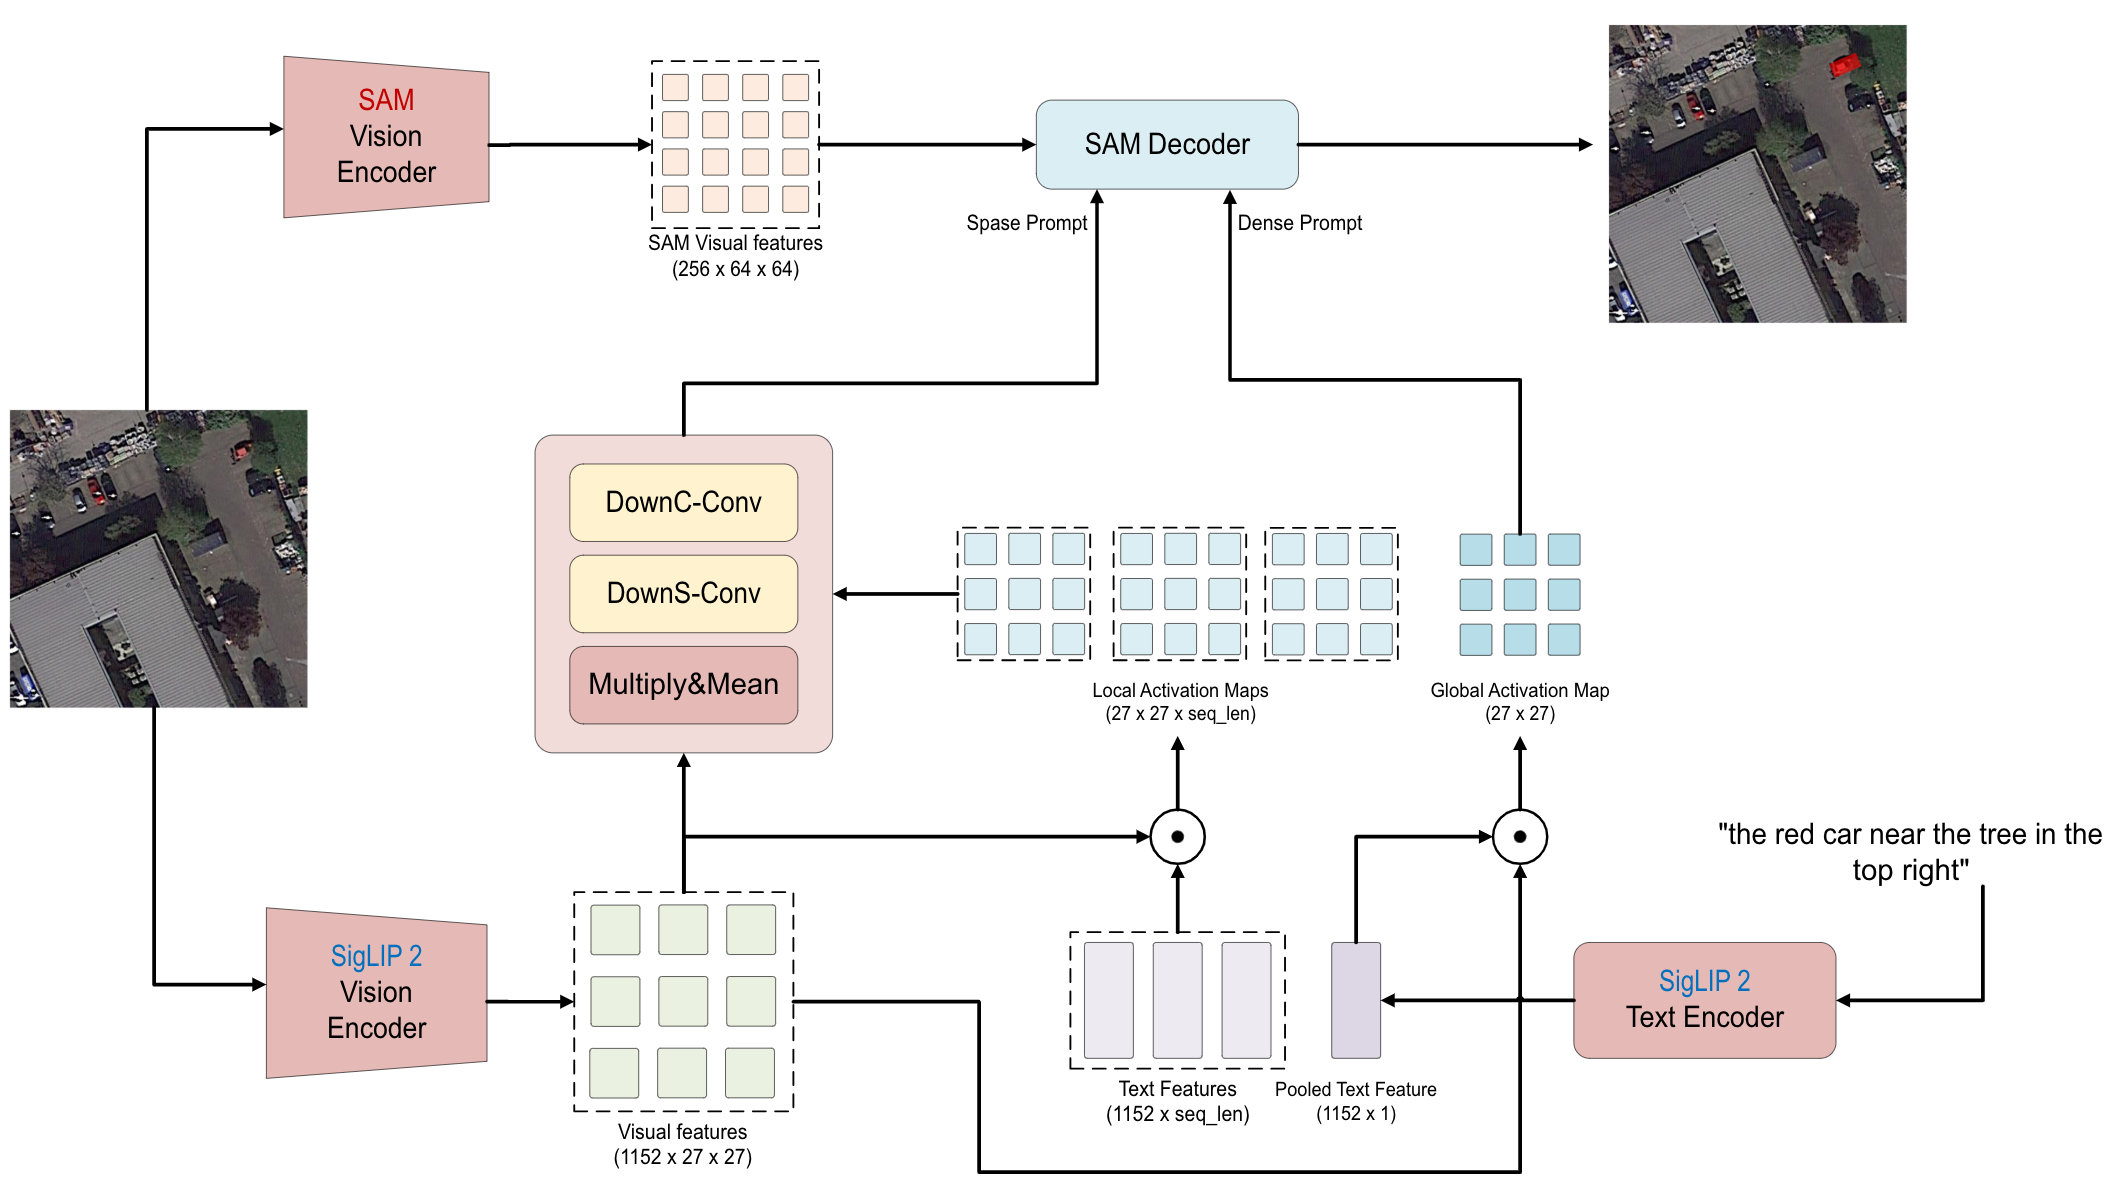
\includegraphics[width=\textwidth]{./Images/clipsam.png}
\caption{RSRefSeg architecture overview showing the integration of SigLIP2 vision-language encoder with SAM mask decoder through custom prompter networks for text-guided segmentation. The dual-pathway design processes both local (token-level) and global (sentence-level) text-visual interactions to generate sparse and dense prompts for precise aerial image segmentation.}
\label{fig:rsrefseg_architecture}
\end{figure}

% #############################################################################
\section{Large Language Models for Vision}

Applications of LLMs to vision tasks and multimodal understanding.

[Reference to GPT architecture and autoregressive generation] % \cite{placeholder_gpt}

[Reference to multimodal capabilities in vision-language models] % \cite{placeholder_multimodal}

[Reference to Gemma 3 open source models with SigLIP vision encoder] % \cite{placeholder_gemma3}

[diagram for Gemma 3 architecture showing Gemma + SigLIP combo for vision capabilities]

[Reference to proprietary API models: O3] % \cite{placeholder_o3}

[Reference to proprietary API models: GPT-5] % \cite{placeholder_gpt5}

[Reference to proprietary API models: Gemini 2.5] % \cite{placeholder_gemini25}

% #############################################################################
\section{Overview}

[Synthesis of all related work - gaps identified and how this work addresses them] % \cite{placeholder_synthesis}